\documentclass[aspectratio = 169, spanish]{beamer}
\usetheme[amurmapleblue]{Amurmaple}

\usepackage[spanish,activeacute,es-noindentfirst]{babel}
%paqueteria para idioma
\spanishdecimal{.}
\usepackage{pstricks}
\usepackage[utf8]{inputenc}
\usepackage{csquotes}
\usepackage{cancel}

%\usepackage{pstricks-add}

\usepackage{mlmodern}
\usepackage[T1]{fontenc}

\usepackage{verbatim}

%Para Figuras en Tikz
\usepackage{tikz}
\usepackage{pgfplots}
\pgfplotsset{compat=1.15}
\usepackage{mathrsfs}

\usepackage{amssymb,amsfonts,amsbsy,amsmath}
\usepackage{graphicx}
\usepackage{mathtools}
\usepackage{amsthm}
\usepackage{dsfont}
\usepackage{float}
\usepackage{enumitem}
% \usepackage[hidelinks]{hyperref}

\usepackage{subfig}

\usepackage{rotating} %para rotar texto en tablas con \begin{sideways}
%\end{sideways}
\usepackage{makecell} %Para dividir celdas de tablas en varias l\'ineas
\usepackage{bm}

% Para creacion de figuras
\usepackage{xcolor}
\usepackage{tikz}

\setbeamertemplate{theorems}[numbered]
\setbeamertemplate{corollary}[numbered]

\newcommand{\E}{\mathbb{E}}

% Titulo
\title[CIMAT 2025]{Regresión no Lineal}
\author[Iván, Rubí, Samuel]{Iván García Mestiza, Jessica Rubí Lara Rosales, Samuel Gurrola Viramontes}
\institute[CIMAT ]{CIMAT}
\date{20 de mayo del 2025}

\AtBeginSection[]
{
    \sectionpage
}

\begin{document}

\maketitle

\begin{frame}

\tableofcontents

\end{frame}

% \begin{frame}
% \sectionpage
% \end{frame}

\section{Introducción}

\begin{frame}{Introducción}
Una tarea importante en estadística es encontrar las relaciones, si existen, en un conjunto de variables cuando al menos una es aleatoria, estando sujeta a fluctuaciones aleatorias y posiblemente a errores de medición.

Usualmente se puede esperar tener una relación del estilo
\begin{align*}
    \bm{y} \approx f(\bm{x}_{1}, \bm{x}_{2}, \ldots, \bm{x}_{k}).
\end{align*}
Sin embargo, los datos frecuentemente contendrán ruido o errores de medición.

\end{frame}

\begin{frame}
    Los modelos de regresión lineal $y = x^T \beta + \varepsilon$ son una herramienta poderosa para cuantificar el impacto de covariables $x$, sobre una respuesta $y$. 
    
    Los modelos de regresión no-lineal extienden estos modelos a \textbf{casos en los que se cuenta con información acerca de la naturaleza del fenómeno}, buscando estimar $\boldsymbol{\theta}$ a partir de la relación
    \begin{align*}
        \boldsymbol{y} = f(\boldsymbol{x}; \boldsymbol{\theta}) + \varepsilon,
    \end{align*}
    en donde $f$ es una función no lineal en $\boldsymbol{\theta}$.
\end{frame}

\begin{frame}{Ejemplo}
\textbf{Modelo exponencial de crecimiento}\\
\vspace{0.5cm}
   Malthus (economista británico) propuso que la \textit{tasa de cambio} de una población con respecto al tiempo es proporcional a la población.
\begin{align*}
    \frac{dy}{dt} = ky.
\end{align*}
Si la población inicial $y(0) = \alpha$, se tiene que la solución es
\begin{align*}
    y = \alpha e^{kt}.
\end{align*}
\end{frame}

\begin{frame}{Ejemplo}
\begin{figure}
    \centering
    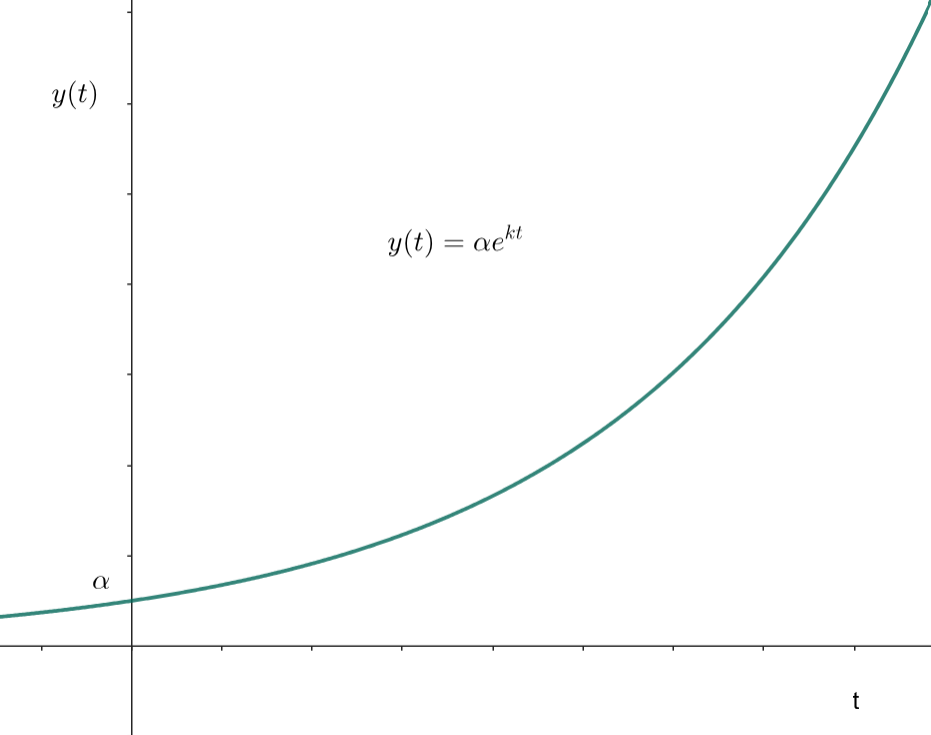
\includegraphics[width=0.5\linewidth]{eje1.png}
    \caption{Crecimiento exponencial}
    \label{fig:ejemplo1}
\end{figure}
\end{frame}


\begin{frame}{Ejemplo}
\begin{figure}
    \centering
    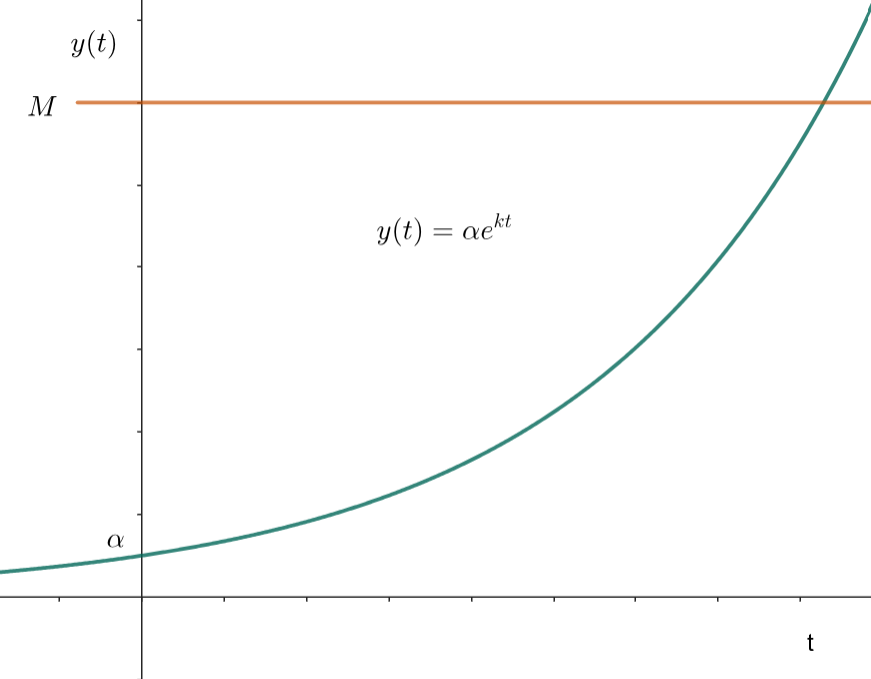
\includegraphics[width=0.5\linewidth]{eje2.png}
    \caption{Crecimiento exponencial con una barrera}
    \label{fig:ejemplo2}
\end{figure}
\end{frame}

\begin{frame}{Ejemplo}
\textbf{Modelo logístico de crecimiento}\\
\vspace{0.5cm}
Verhulst consideró una variante en la que el ambiente no puede soportar más que cierta población máxima $M$, así que la población crece de manera acelerada y  a partir de cierto punto el tamaño de la población se ralentiza. 
\begin{align*}
    \frac{d y}{d t} = k y \left(1 - \frac{y}{M}\right).
\end{align*}
donde $y(t) \to M$ cuando $t \to \infty$. Suponiendo que $y(0) = \alpha$, usando el método de separación de variables obtenemos
\begin{align*}
    y(t) = \frac{\alpha M}{(M - \alpha) e^{-kt} + \alpha} = \frac{ M}{e^{-k(t - t_0)} + 1}
\end{align*}
El modelo logístico, con su característico comportamiento sigmoidal es muy utilizado como modelo de crecimiento. 
\end{frame}

\begin{frame}{Ejemplo}
    \begin{figure}
        \centering
        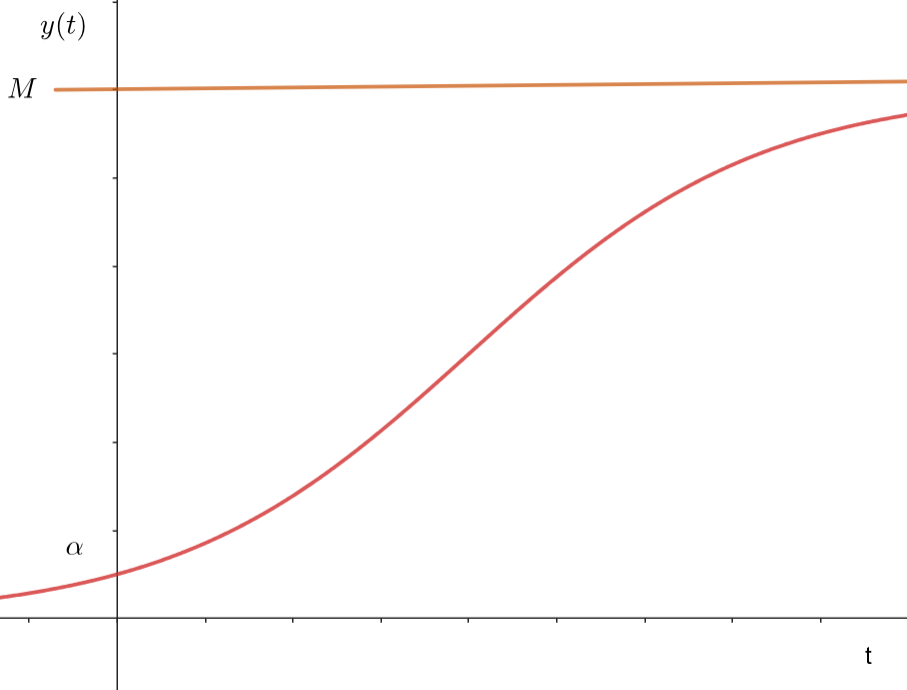
\includegraphics[width=0.5\linewidth]{eje3.png}
        \caption{Crecimiento logístico}
        \label{fig:ejemplo3}
    \end{figure}
\end{frame}

\begin{frame}{Ejemplo }
Base de datos del INEGI de las personas (nacionales o extranjeros) que residen en México.
    \begin{figure}[htbp]
    \begin{minipage}[c]{0.3\textwidth}
    {\tiny \begin{tabular}{|c|c|}
            \hline Año & Población en México\\
            \hline
            1910 & 15160369\\
            1921 &  14334780\\
            1930 & 16552722\\
            1940 & 19653552\\
            1950 & 25791017\\
            1960 & 34923129\\
            1970 & 48225238\\
            1980 & 66846833\\
            1990 & 81249645\\
            1995 & 91158290\\
            2000 & 97483412\\
            2005 & 103263388\\
            2010 & 112336538\\
            2015 & 119938473\\
            2020 & 126014024 \\ \hline
        \end{tabular}}
        \end{minipage}
        \begin{minipage}[c]{0.65\textwidth}
         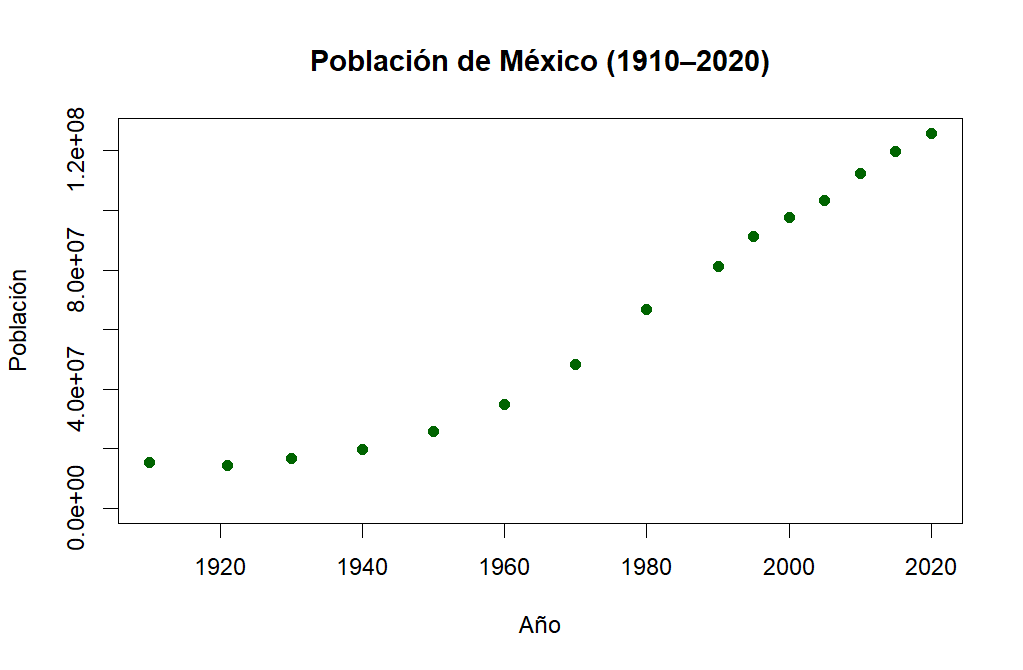
\includegraphics[width=\linewidth]{poblacion1.png}
        \end{minipage}
    \end{figure}
       
\end{frame}

\begin{frame}{Ejemplo}
    \begin{align*}
        y(t) = \frac{M}{1 + e^{-k(t - t_0)}}\hspace{1cm} M = 181,900,000, \ k=0.03583 \hspace{0.2cm}\text{y}\hspace{0.2cm}t_0 = 1997
    \end{align*}
    \begin{center}
        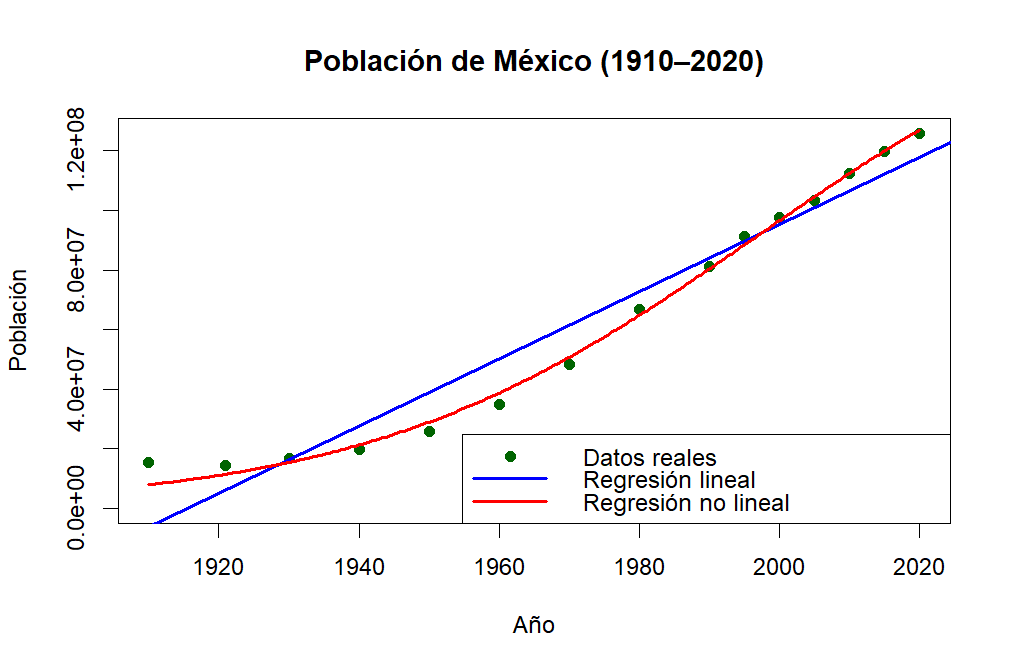
\includegraphics[scale=0.6]{logis1.png}
    \end{center}
    
\end{frame}

\begin{frame}{Modelo de Regresión No Lineal}
En general, escribiremos el modelo de regresión no lineal como
\[
    y = f\left(\bm{x}, \boldsymbol{\theta}\right) + \varepsilon
\]
\begin{itemize}
    \item $y$ variable de respuesta o dependientes.
    \item $\bm{x}$ variable explicativa o regresora.
    \item \(\boldsymbol{\theta} = (\theta_1, \ldots, \theta_p)^\top\) es un vector de tamaño \(p \times 1\) de parámetros desconocidos.
    \item $f$ es una función no lineal de los parámetros.
    \item  \(\varepsilon\) es un término de error aleatorio no correlacionado con $\varepsilon \sim N(0, \sigma^2)$.
\end{itemize}
Dado que
\begin{align*}
    \mathbb E\left(\bm{y}\right) &= \mathbb E\left[f\left(\bm{x}, \boldsymbol{\theta}\right) + \varepsilon\right]\\
&= f\left(\bm{x}, \boldsymbol{\theta}\right)
\end{align*}
llamamos a \(f(\bm{x}, \boldsymbol{\theta})\) la \textbf{función de respuesta esperada}.
\end{frame}


\begin{frame}{No linealidad}
    \textbf{Lineal}\\
   \begin{align*}
    \bm{y} = \beta_{0} + \beta_{1}\bm{z}_{1} + \cdots + \beta_{p-1}\bm{z}_{p-1} + \bm\varepsilon,
    \end{align*}
    se admiten transformaciones como $x_ix_j$, $\exp(x_i)$, $\sqrt{x_i}$ y $\sin(x_i)$. Son lineales en los parámetros desconocidos $\beta_i$, $i = 1, 2, \ldots, p$.\\
    \vspace{0.5cm}
    \textbf{No Lineal}\\
    \begin{align*}
        y = \theta_1 e^{ \theta_2 x} + \varepsilon, \hspace{1cm} y= \frac{\theta_1 \theta_3}{(\theta_3 - \theta_1) e^{-\theta_2 x} + \theta_1} + \varepsilon
    \end{align*}
    No lineal en los parámetros 
\end{frame}

\begin{frame}{Verificación no linealidad}
    \[
    \bm y = f\left(\bm{x},\bm{\beta}\right) + \bm \varepsilon = \beta_{0} + \sum_{j=1}^{k}\beta_{j}x_{j} + \bm \varepsilon.
\]

Ahora,
\[
\frac{\partial f\left(\bm{x},\bm{\beta}\right)}{\partial\beta_{j}} = x_{j}, \quad j=0,1, \ldots, k,
\]
donde $\bm x_{0} \equiv 1$. Nótese que en el caso lineal las derivadas son constantes con respecto a $\bm{\beta}$.

Por otro lado, consideremos el modelo no lineal
\[
y = f\left(x,\bm{\theta}\right) + \varepsilon = \theta_{1}e^{\theta_{2}x} + \varepsilon.
\]
Las derivadas de la función expectativa con respecto a $\theta_{1}$ y $\theta_{2}$ son:
\[
\frac{\partial f\left(x,\bm{\theta}\right)}{\partial\theta_{1}} = e^{\theta_{2}x} \quad \text{y} \quad \frac{\partial f\left(x,\bm{\theta}\right)}{\partial\theta_{2}} = \theta_{1}xe^{\theta_{2}x}.
\]
Dado que las derivadas son función de los parámetros desconocidos $\theta_{1}$ y $\theta_{2}$, el modelo es no lineal.
\end{frame}


\section{Métodos de Estimación}

\begin{frame}{Transformación a modelos lineales}
A veces es útil considerar una \textbf{transformación} que induzca linealidad en la función de expectativa del modelo. Por ejemplo, en el modelo
\begin{align}\label{linea1}
    y = f(x, \bm\theta) + \varepsilon = \theta_1 e^{\theta_2 x} + \varepsilon
\end{align}
se tiene que $\E(y) = f(x, \theta) = \theta_1 e^{\theta_2 x}$, por lo que podemos linealizar la función de expectativa tomando logaritmos:
\[
\ln \E(y) = \ln \theta_1 + \theta_2 x.
\]
\end{frame}

\begin{frame}
    Luego, podemos pensar en ajustar el modelo
    \begin{align}\label{linea2}
        \ln y = \ln \theta_1 + \theta_2 x + \varepsilon = \beta_0 + \beta_1 x + \varepsilon
    \end{align}
    y usar regresión lineal simple para estimar $\beta_0$ y $\beta_1$.

    Sin embargo, en general las estimaciones de los parámetros bajo transformaciones no son equivalentes a las estimaciones del modelo general.

     Además, en la ecuación \eqref{linea1} la estructura del error es aditiva, por lo que tomar logaritmos no puede producir el modelo en la ecuación \eqref{linea2}.
\end{frame}

\begin{frame}
   Si la estructura del error es multiplicativa, por ejemplo
    \[
    y = \theta_1 e^{\theta_2 x} \varepsilon
    \]
    entonces tomar logaritmos será apropiado, ya que
    \[
    \ln y = \ln \theta_1 + \theta_2 x + \ln \varepsilon = \beta_0 + \beta_1 x + \varepsilon^*
    \]
    y si $\varepsilon^*$ sigue una distribución normal, todas las propiedades estándar del modelo de regresión lineal y la inferencia asociada serán aplicables.

    El problema a menudo gira en torno a la estructura del error: ?`se aplican los supuestos estándar sobre los errores al modelo no lineal original o al linealizado?
\end{frame}

\begin{frame}{Modelo de Michaelis–Menten}
    El modelo de \textbf{Michaelis–Menten} es un modelo de cinética química que relaciona la velocidad inicial de una reacción enzimática con la concentración de sustrato $x$. Dicho modelo es 
    \begin{equation}\label{Eq-Puromicina}
        y = \frac{\theta_1 x}{x+\theta_2}+\varepsilon.
    \end{equation}
    
    Se tienen datos de la velocidad inicial de una reacción para una enzima tratada con puromicina, y se desean estimar los coeficientes $\theta_1$ y $\theta_2$.
\end{frame}

\begin{frame}
    \begin{center}
        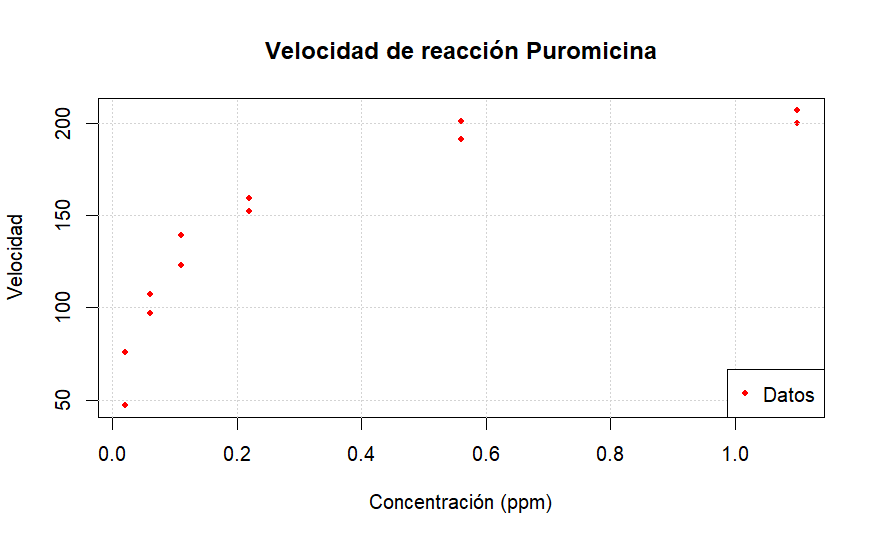
\includegraphics[scale=0.65]{puromicina1.png}
    \end{center}
\end{frame}

\begin{frame}
    La función de respuesta esperada puede ser linealizada fácilmente como sigue:
    \[
    \frac{1}{f(x, \boldsymbol{\theta)}} = \frac{x+\theta_2}{\theta_1 x} = \frac{1}{\theta_1} + \frac{\theta_2}{\theta_1}x.
    \]
    Por lo tanto, un primer acercamiento es ajustar el modelo lineal
    \[
    y^\star = \beta_0 + \beta_1 u + \varepsilon,
    \]
    en donde $y^\star = 1/y$ y $u = 1/x$. El modelo lineal ajustado resulta ser:
    \[
    y^\star = 0.0051072 + 0.0002472 u.
    \]
\end{frame}

\begin{frame}
    \begin{center}
        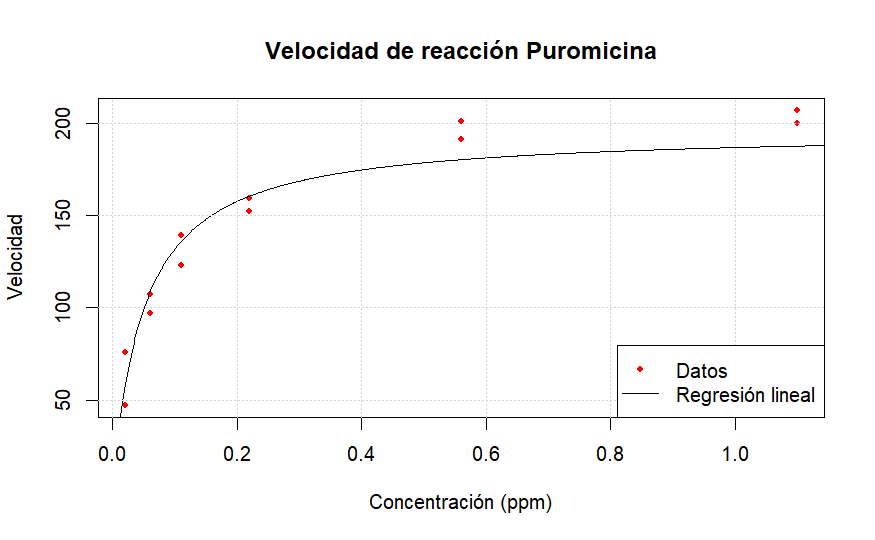
\includegraphics[scale=0.65]{puromicina2.png}
    \end{center}
\end{frame}

\begin{frame}
    \begin{center}
        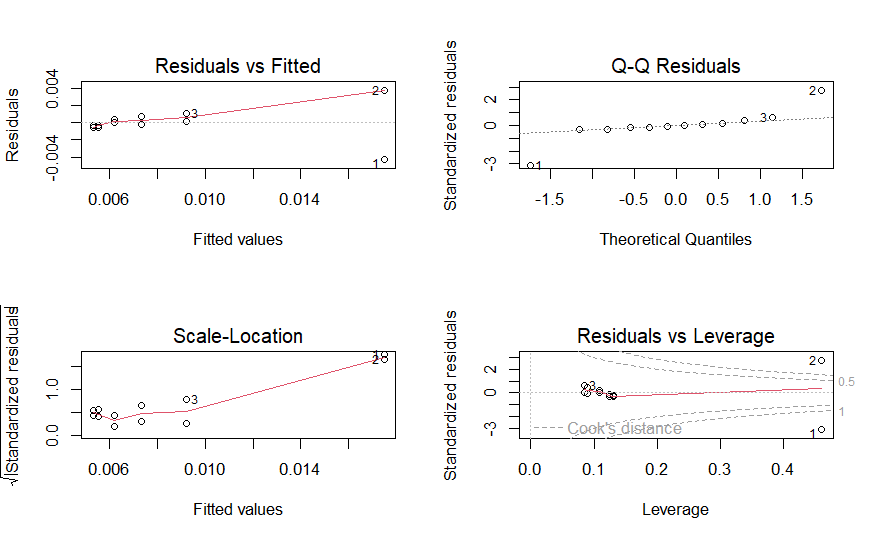
\includegraphics[scale=0.65]{puromicina3.png}
    \end{center}    
\end{frame}

\begin{frame}
    Al hacer una prueba de Anderson-Darling, obtenemos un p-valor de $0.006107$, y como se puede observar en las gráficas anteriores, el ajuste no es muy bueno.
    
    El modelo lineal tiene como parámetros ajustados $\theta_1 = 195.80270885$ y $\theta_2 = 0.04840653$. Posteriormente se verá su relación con los parámetros obtenidos al realizar regresión no lineal.
\end{frame}

\begin{frame}{Mínimos cuadrados no lineales}
El modelo no lineal es
\[
y_{i} = f\left( \bm{x}_{i}, \bm{\theta} \right) + \varepsilon_{i}, \quad i=1,2,\ldots,n,
\]
donde ahora $\bm{x}_{i} = (x_{i1}, x_{i2}, \ldots, x_{ik})$ para $i=1,2,\ldots,n$. La función de mínimos cuadrados es
\[
S(\bm{\theta}) = \sum_{i=1}^{n} \left( y_{i} - f\left( \bm{x}_{i}, \bm{\theta} \right) \right)^{2}.
\]
Diferenciamos la ecuación anterior con respecto a cada elemento de $\bm{\theta}$, lo cual proporcionará un conjunto de $p$ ecuaciones normales para la situación de regresión no lineal, que son:
\[
\sum_{i=1}^{n} \left( y_{i} - f\left( \bm{x}_{i}, \bm{\theta} \right) \right) {\left[ \frac{\partial f\left( \bm{x}_{i}, \bm{\theta} \right)}{\partial \theta_{j}} \right]}_{\bm{\theta} = \hat{\bm{\theta}}} = 0 \quad \text{para } j=1,2,\ldots,p.
\]
\end{frame}


\begin{frame}{Ejemplo}
    Consideremos el modelo de regresión no lineal
\[
y = \theta_1 e^{\theta_2 x} + \varepsilon.
\]
Las ecuaciones normales de mínimos cuadrados para este modelo son
\begin{align*}
    \sum_{i=1}^{n} \left( y_i - \hat{\theta}_1 e^{\hat{\theta}_2 x_i} \right) e^{\hat{\theta}_2 x_i} = 0,\hspace{1cm}
\sum_{i=1}^{n} \left( y_i - \hat{\theta}_1 e^{\hat{\theta}_2 x_i} \right) \hat{\theta}_1 x_i e^{\hat{\theta}_2 x_i} = 0.
\end{align*}
Después de simplificar, las ecuaciones normales quedan:

\begin{align*}
     \sum_{i=1}^{n} y_i e^{\hat{\theta}_2 x_i} - \hat{\theta}_1 \sum_{i=1}^{n} e^{2\hat{\theta}_2 x_i} = 0,\hspace{1cm}\sum_{i=1}^{n} y_i x_i e^{\hat{\theta}_2 x_i} - \hat{\theta}_1 \sum_{i=1}^{n} x_i e^{2\hat{\theta}_2 x_i} = 0.
\end{align*}
   
Estas ecuaciones no son lineales en $\hat{\theta}_1$ y $\hat{\theta}_2$, y no existe una solución cerrada simple.

\end{frame}

\begin{frame}{Mínimos cuadrados no lineales}
    \textbf{Nota: }
\begin{itemize}
    \item Las derivadas de la función de respuesta esperada serán funciones de los parámetros desconocidos.
    \item La función $f$ también es una función no lineal, por lo que las ecuaciones normales pueden ser muy difíciles de resolver.
    \item Al igual que en el modelo de regresión lineal, se espera que el número de datos $n$ sea mayor que el número de parámetros a estimar $p$.
\end{itemize}
\end{frame}
\begin{frame}{Máxima Verosimilitud}
Como los errores $\varepsilon_i \sim N(0, \sigma^2)$ son iid, la función de verosimilitud es:
\[
L(\bm\theta, \sigma^2) = \frac{1}{(2\pi\sigma^2)^{n/2}} \exp\left[ -\frac{1}{2\sigma^2} \sum_{i=1}^n \left[y_i - f(\bm{x}_i; \bm{\theta})\right]^2 \right].
\]
Maximizar esta función de verosimilitud es equivalente a minimizar la suma de cuadrados residuales. Por lo tanto, las estimaciones por mínimos cuadrados son iguales a las estimaciones de máxima verosimilitud.
\end{frame}

\begin{frame}{Geometría de Mínimos Cuadrados Lineales y No Lineales}
\begin{center}
     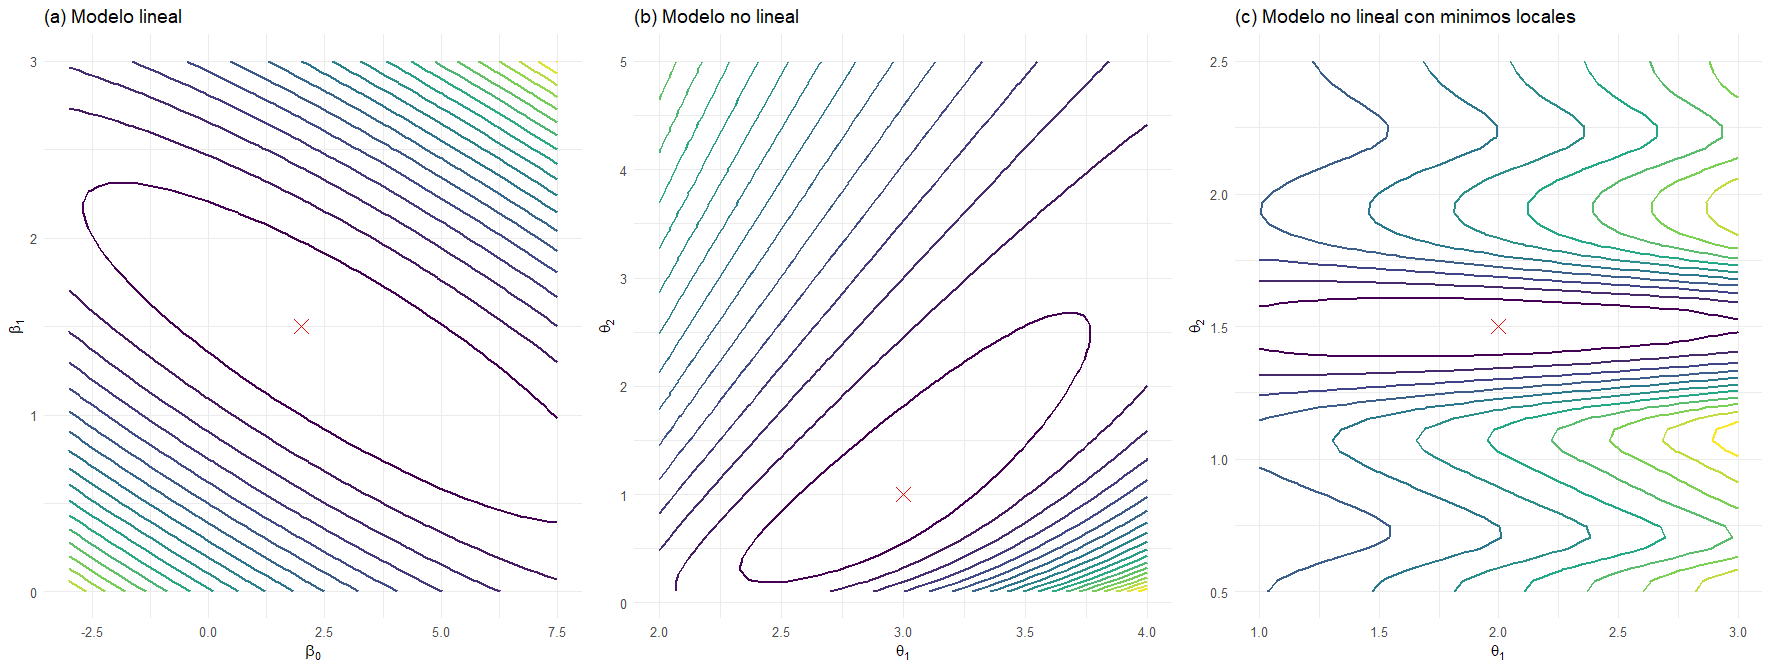
\includegraphics[scale=0.46]{proy1.png}
\end{center}
   
\end{frame}



\begin{frame}{Estimación de parámetros en modelos no lineales}
    Un método ampliamente utilizado en algoritmos computacionales para regresión no lineal es la \textbf{linealización} de la función no lineal seguida de algún método para estimación de parámetros.

    Se logra mediante una expansión en \textbf{series de Taylor} de $f(\bm x_i, \bm\theta)$ alrededor del punto $\bm\theta_0 = (\theta_{1}^{0}, \theta_{2}^{0}, \ldots, \theta_{p}^{0})$, conservando sólo los términos lineales. De aquí se obtiene el modelo aproximado
    \begin{equation}\label{Eq1-Sec1.3.1}
        f(\bm{x}_i, \bm{\theta}) \approx f(\bm{x}_i, \bm{\theta}_0) + \sum_{j=1}^p \left[ \frac{\partial f(\bm{x}_i, \bm{\theta})}{\partial \theta_j} \right]_{\bm{\theta} = \bm{\theta}_0} (\theta_j - \theta_{j}^{0}).
    \end{equation}
\end{frame}

\begin{frame}
    Si definimos
\[
\begin{split}
    f_i^0 &= f(\bm{x}_i, \bm{\theta}_0),\\
    \beta_j^0 &= \theta_j - \theta_{j}^{0},\\
    X_{ij}^0 &= \left[ \frac{\partial f(\bm{x}_i, \bm{\theta})}{\partial \theta_j} \right]_{\bm{\theta} = \bm{\theta}_0},
\end{split}
\]
observamos que el modelo de regresión no lineal puede escribirse como:
\begin{equation}\label{Eq2-Sec1.3.1}
    y_i - f_i^0 = \sum_{j=1}^{p} \beta_j^0 X_{ij}^0 + \varepsilon_i, \quad i = 1, 2, \ldots, n.
\end{equation}
Es decir, ahora tenemos un modelo de regresión lineal.
\end{frame}

\begin{frame}
    Podemos escribir la ecuación (\ref{Eq2-Sec1.3.1}) como
\[
\bm{y}_{0} = {X}_0 \bm{\beta}_{0} + \bm{\varepsilon},
\]
por lo que la estimación de $\bm{\beta}_{0}$ es
\begin{equation}\label{Eq-Incrementos-Gauss-Newton}
    \bm{\hat{\beta}}_0 = ({X}_0^\top {X}_0)^{-1} {X}_0^\top \bm{y}_0 = ({X}_0^\top {X}_0)^{-1} {X}_0^\top (\bm{y} - \bm{f}_0)
\end{equation}

Dado que $\bm{\beta}^{0} = \bm{\theta} - \bm{\theta}_{0}$, definimos
\[
\bm{\hat{\theta}}_1 = \bm{\hat{\beta}}_0 + \bm{\theta}_0
\]
como las nuevas estimaciones de $\bm{\theta}$. A $\bm{\hat{\beta}}_0$ también se le conoce como \textbf{vector de incrementos}.
\end{frame}

\begin{frame}
    Podemos usar las nuevas estimaciones $\bm{\hat{\theta}}_1$ en la ecuación (\ref{Eq1-Sec1.3.1}) para producir otro conjunto de estimaciones, digamos $\bm{\hat{\theta}}_2$, y así sucesivamente.

En general, en la $k$-ésima iteración tenemos:
\begin{equation}\label{Eq-Incrementos.Sec1.3.1}
    \bm{\hat{\theta}}_{k+1} = \bm{\hat{\theta}}_k + \bm{\hat{\beta}}_k = \bm{\hat{\theta}}_k + ({X}_k^\top {X}_k)^{-1} {X}_k^\top (\bm{y} - \bm{f}_k),
\end{equation}
donde
\[
\begin{split}
    {X}_k &= [X_{ij}^k],\\
    \bm{f}_k &= {[f_1^k, f_2^k, \ldots, f_n^k]}^\top,\\
    \bm{\hat{\theta}}_k &= {[\theta_{1}^k, \theta_{2}^k, \ldots, \theta_{p}^k]}^\top.
\end{split}
\]
\end{frame}

\begin{frame}
    Este proceso iterativo continúa hasta alcanzar la convergencia, es decir, hasta que
\[
\frac{\hat{\theta}_{j}^{k+1} - \hat{\theta}_{j}^{k}}{\hat{\theta}_{j}^{k}} < \delta, \quad j = 1, 2, \ldots, p,
\]
donde $\delta$ es un número pequeño, por ejemplo $1.0 \times 10^{-6}$. 

En cada iteración se debe evaluar la suma de cuadrados residual $S(\bm{\hat{\theta}}_k)$ para asegurar que se ha obtenido una reducción en su valor.
\end{frame}


\begin{frame}{Ejemplo Puromicina}
    Podemos hacer los cálculos anteriores para el ejemplo de Puromicina como sigue: Tomando los valores iniciales $\theta_{10} = 205$ y $\theta_{20} = 0.08$, se tiene la suma de cuadrados residual $S(\bm{\theta}_0) = 3155$.

    \[
    \frac{\partial f(x, \theta_1, \theta_2)}{\partial \theta_1} = \frac{x}{\theta_2 + x} \quad \text{y} \quad \frac{\partial f(x, \theta_1, \theta_2)}{\partial \theta_2} = \frac{-\theta_1 x}{\left(\theta_2 + x\right)^2}
    \]
    Como la primera observación de $x$ es $x_1 = 0.02$, tenemos:
    \[
    X_{11}^0 = \left. \frac{x_1}{\theta_2 + x_1} \right|_{\theta_2 = 0.08} = \frac{0.02}{0.08 + 0.02} = 0.2,
    \]
    y también,
    \[
    X_{12}^0 = \left. \frac{-\theta_1 x_1}{\left(\theta_2 + x_1\right)^2} \right|_{\substack{\theta_1 = 205 \\ \theta_2 = 0.08}} = \frac{(-205)(0.02)}{\left(0.08 + 0.02\right)^2} = -410.
    \]
\end{frame}

\begin{frame}
    Las derivadas $X_{ij}^0$ se recopilan en la matriz $\bm{X}_0$ y el vector de incrementos se calcula a partir de la ecuación (\ref{Eq-Incrementos-Gauss-Newton}) como:
\[
\hat{\bm{\beta}}_0 = \begin{bmatrix}
8.03 \\
-0.017
\end{bmatrix}.
\]
La nueva estimación de $\hat{\bm{\theta}}_1$ a partir de la ecuación (\ref{Eq-Incrementos.Sec1.3.1}) es:
\[
\hat{\bm{\theta}}_1 = \hat{\bm{\beta}}_0 + \bm{\theta}_0
=
\begin{bmatrix}
8.03 \\
-0.017
\end{bmatrix} +
\begin{bmatrix}
205.00 \\
0.08
\end{bmatrix}
=
\begin{bmatrix}
213.03 \\
0.063
\end{bmatrix}.
\]
\end{frame}

\begin{frame}
    La suma de cuadrados residual en este punto es $S(\hat{\bm{\theta}}_1) = 1206$, que es considerablemente menor que $S(\bm{\theta}_0)$. Por lo tanto, $\hat{\bm{\theta}}_1$ se adopta como la nueva estimación de $\bm{\theta}$, y se realizaría otra iteración.

El algoritmo Gauss-Newton converge en $\hat{\bm{\theta}}^\top = [212.7,\, 0.0641]^\top$ con $S(\hat{\bm{\theta}}) = 1195$. Así, el modelo ajustado obtenido por linealización es:
\[
\hat{y} = \frac{\hat{\theta}_1 x}{x + \hat{\theta}_2} = \frac{212.7 x}{x + 0.0641}.
\]
Estos cálculos pueden realizarse automáticamente con la función nls() de R.
\end{frame}

\begin{frame}
    \begin{center}
        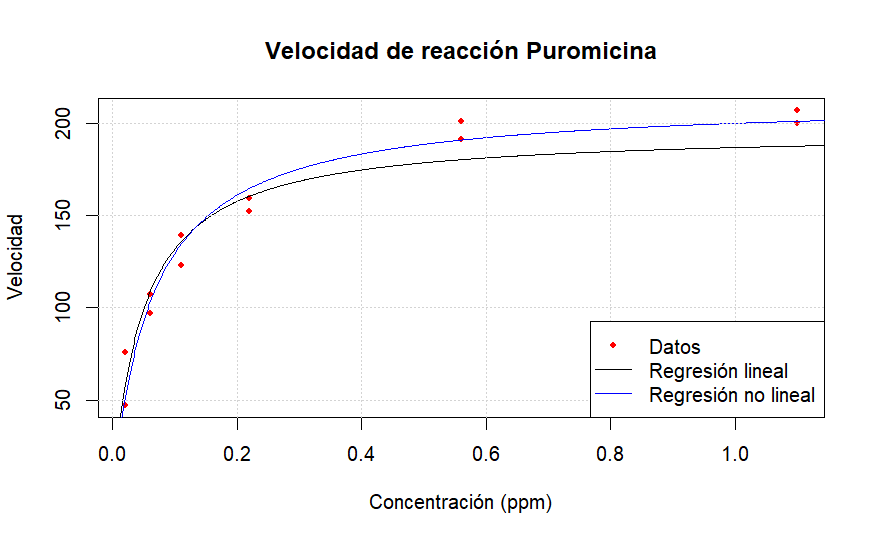
\includegraphics[scale=0.6]{puromicina4.png}
    \end{center}
\end{frame}

\begin{frame}{Perspectiva gráfica de linealización}
    \begin{center}
        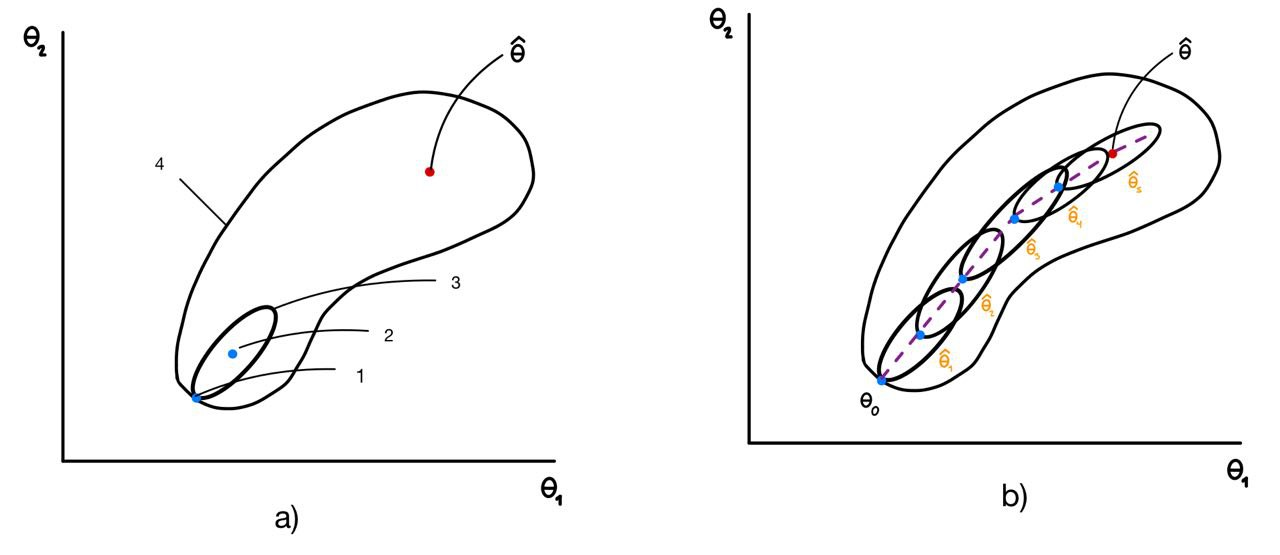
\includegraphics[scale=0.28]{proy2.jpg}
    \end{center}
{\small\begin{itemize}
    \item Valor inicial $\bm{\theta}_0$
    \item Primera iteración de la solución linealizada $\hat{\bm{\theta}}_1$
    \item Suma residual del contorno de secuencias en el problema linealizado
    \item $S(\bm\theta)$ contorno pasando a través de $\bm\theta$.
\end{itemize}
}
\end{frame}


\begin{frame}{Estimación de la Varianza}
    Cuando el procedimiento de estimación converge a un vector final de estimaciones de parámetros $\hat{\theta}$, podemos obtener una estimación de la varianza del error $\sigma^2$ mediante el error cuadrático medio
\[
\hat{\sigma}^2 = MS_{\text{Res}} = \frac{\sum_{i=1}^{n}(y_i - \hat{y}_i)^2}{n-p} = \frac{\sum_{i=1}^{n}\left[y_i - f(\bm{x}_i, \bm{\hat{\theta}})\right]^2}{n-p} = \frac{S(\bm{\hat{\theta}})}{n-p},
\]
También podemos estimar la \textbf{matriz de covarianzas asintótica} (para muestras grandes) del vector de parámetros $\bm{\hat{\theta}}$ como
\begin{equation}\label{Eq-Var-asintotica}
    \operatorname{Var}(\bm{\hat{\theta}})=\sigma^2 {\left(\hat{X}^\top \hat{X}\right)}^{-1},
\end{equation}
en donde $\hat{X}$ es la matriz de derivadas parciales definida previamente, evaluada en la última iteración del estimador de mínimos cuadrados $\bm{\hat{\theta}}$.
\end{frame}

\begin{frame}{Método de Descenso de Gradiente}
Este método se basa en una aproximación cuadrática a la función objetivo, en este caso $S(\bm{\theta})$. Supongamos que $\bm{\theta}_0$ es un valor inicial cercano al valor óptimo. Entonces, podemos aproximar $S(\bm{\theta})$ mediante una expansión de Taylor de segundo orden alrededor de $\bm{\theta}_0$:
\[
S(\bm{\theta}) \approx S(\bm{\theta}_0) + (\bm{\theta} - \bm{\theta}_0)^\top \nabla S(\bm{\theta}_0) + \frac{1}{2} (\bm{\theta} - \bm{\theta}_0)^\top H_S(\bm{\theta}_0) (\bm{\theta} - \bm{\theta}_0),
\]
\end{frame}

\begin{frame}{Método de Newton-Rapshon}
\end{frame}

\begin{frame}
    Gráficas de convergencia de métodos iterativos \textbf{SAMUEL} (comparar descenso máximo, incrementos fraccionarios, Marquardt)
\end{frame}

\begin{frame}{Valores iniciales}
    
\end{frame}

\section{Inferencia estadística en regresión no lineal}

\begin{frame}
    Intro al tema
\end{frame}

\begin{frame}{Regiones de confianza}
    
\end{frame}

\begin{frame}{Validez de la inferencia aproximada}
    
\end{frame}

\section{Validación del modelo}

\begin{frame}{Comparación de modelos}
    
\end{frame}

\begin{frame}{Medidas de ajuste}
    
\end{frame}

\begin{frame}{Medidas de no linealidad}
    
\end{frame}


\section{Conclusiones}

\begin{frame}{Conclusiones}
    Ventajas y desventajas, incluyendo no identificabilidad
\end{frame}

\begin{frame}{Referencias}
    
\end{frame}

\end{document}
